% SecretHandle — ACM MobiSys Full Research Paper submission draft
% Single-blind: real author names included.
% Build: xelatex main.tex (x2) ; bibtex main ; xelatex main.tex (x2)
\documentclass[sigconf,10pt]{acmart}

\usepackage{microtype}
\usepackage{booktabs}
\usepackage{tabularx}
\usepackage{enumitem}
\usepackage{amsmath}
\usepackage{algorithm}
\usepackage{algpseudocode}
\usepackage{tikz}
\usepackage{pgfplots}
\pgfplotsset{compat=1.18}
\usetikzlibrary{arrows.meta,positioning,calc,fit,backgrounds,shapes.geometric,shapes.symbols,decorations.pathreplacing,patterns,matrix}
\definecolor{shblue}{HTML}{2F6B9A}
\definecolor{shbluefill}{HTML}{DCECF7}
\definecolor{shorange}{HTML}{C65D20}
\definecolor{shorangefill}{HTML}{FBE3D3}
\definecolor{shgreen}{HTML}{2E7D5B}
\definecolor{shgreenfill}{HTML}{DDF1E7}
\definecolor{shpurple}{HTML}{6C4AA1}
\definecolor{shpurplefill}{HTML}{E9E0F5}
\definecolor{shgray}{HTML}{5F6770}
\definecolor{shgrayfill}{HTML}{EEF0F2}
\tikzset{
  sh/component/.style={draw=shblue,fill=shbluefill,rounded corners=2pt,thick,minimum width=25mm,minimum height=11mm,align=center,font=\small},
  sh/source/.style={draw=shgray,fill=shgrayfill,rounded corners=2pt,thick,minimum width=22mm,minimum height=10mm,align=center,font=\small,pattern=north east lines,pattern color=gray!25},
  sh/defense/.style={draw=shgreen,fill=shgreenfill,rounded corners=2pt,thick,minimum width=27mm,minimum height=11mm,align=center,font=\small},
  sh/attack/.style={draw=shorange,fill=shorangefill,diamond,aspect=2.2,thick,align=center,font=\small},
  sh/theory/.style={draw=shpurple,fill=shpurplefill,rounded corners=2pt,thick,minimum width=28mm,minimum height=10mm,align=center,font=\small},
  sh/infrastructure/.style={draw=shgray,fill=shgrayfill,rounded corners=2pt,thick,minimum width=25mm,minimum height=10mm,align=center,font=\small},
  sh/flow/.style={-{Latex[length=2.2mm]},thick,draw=shblue,shorten >=2pt,shorten <=2pt},
  sh/secureflow/.style={-{Latex[length=2.2mm]},thick,draw=shgreen,shorten >=2pt,shorten <=2pt},
  sh/attackflow/.style={-{Latex[length=2.2mm]},thick,dashed,draw=shorange,shorten >=2pt,shorten <=2pt},
  sh/control/.style={-{Latex[length=2mm]},semithick,densely dotted,draw=shgray,shorten >=2pt,shorten <=2pt},
  sh/label/.style={midway,fill=white,inner sep=1.5pt,font=\scriptsize,align=center},
  sh/group/.style={draw=shgray,dashed,rounded corners=4pt,inner sep=5pt}
}


\newcommand{\SH}{\textsc{SecretHandle}}
\newcommand{\Enter}{\ensuremath{\mathsf{Enter}}}
\newcommand{\Mint}{\ensuremath{\mathsf{Mint}}}
\newcommand{\Resolve}{\ensuremath{\mathsf{Resolve}}}
\newcommand{\Redact}{\ensuremath{\mathsf{Redact}}}
\newcommand{\Reject}{\ensuremath{\mathsf{Reject}}}
\newcommand{\Adv}{\ensuremath{\mathsf{Adv}}}
\newcommand{\Match}{\ensuremath{\mathsf{Match}}}
\newcommand{\View}{\ensuremath{\mathsf{View}}}
\newcommand{\Real}{\ensuremath{\mathsf{Real}}}
\newcommand{\bits}{\{0,1\}}
\newcommand{\sample}{\leftarrow_{\$}}
\newcommand{\enc}{\ensuremath{\mathsf{enc}}}
\newcommand{\cmark}{\tikz[baseline=-0.5ex]\draw[line width=0.2ex,line cap=round,line join=round] (0,0.08) -- (0.07,-0.05) -- (0.22,0.16);}
\newcommand{\xmark}{\ensuremath{\times}}
\newcommand{\pmark}{\ensuremath{\circ}}

% acmart creates theorem/definition/proposition/lemma/corollary in \AtEndPreamble,
% so define the extra environments after they exist.
\AtEndPreamble{%
  \theoremstyle{acmplain}%
  \newtheorem{assumption}[theorem]{Assumption}%
  \newtheorem{remark}[theorem]{Remark}%
}

\settopmatter{printacmref=false,printfolios=true}
\renewcommand\footnotetextcopyrightpermission[1]{}
\acmConference[MobiSys '27]{The 25th Annual International Conference on Mobile Systems, Applications and Services}{June 21--25, 2027}{Ho Chi Minh City, Vietnam}
\acmYear{2027}
\acmDOI{}
\acmISBN{}
\setlength{\emergencystretch}{3em}
\setlength{\textfloatsep}{8pt plus 2pt minus 2pt}
\setlength{\floatsep}{6pt plus 2pt minus 2pt}
\setlength{\intextsep}{6pt plus 2pt minus 2pt}
\setlength{\dbltextfloatsep}{8pt plus 2pt minus 2pt}
\setlength{\abovecaptionskip}{5pt plus 1pt minus 1pt}
\setlength{\belowcaptionskip}{2pt plus 1pt minus 1pt}

\begin{document}

\title[SecretHandle]{SecretHandle: OS-Minted, Destination- and Task-Bound Opaque Secrets\\ for Android Mobile AI Agents}

\author{Nguyễn Tiến Thuận}
\email{thuanntce181024@fpt.edu.vn}
\affiliation{%
  \institution{FPT University}
  \city{Can Tho}
  \country{Vietnam}}

\author{Trần Phát Tài}
\email{taitpce181632@fpt.edu.vn}
\affiliation{%
  \institution{FPT University}
  \city{Can Tho}
  \country{Vietnam}}

\renewcommand{\shortauthors}{Nguyễn and Trần}

\begin{abstract}
Mobile GUI agents must often use a one-time password, credential, address, phone number, or payment identifier to finish a task. Today the value is placed in a screenshot, accessibility tree, prompt, or action argument, so an injected instruction can convert task authority into disclosure or redirection. We present \SH, an Android design for \emph{usable but invisible} secrets: a privileged service mints an opaque, authenticated handle at the authoritative OS source---the SMS or notification OTP pipeline, Credential Manager, the clipboard, or a wallet---before the raw value can reach the agent. The handle binds a secret type, a task identifier, a destination predicate over package and field class (with fail-closed confinement for unattested WebViews), and a type-specific lifecycle (single-use and TTL for OTPs, task-scoped for identifiers, confirm-per-use for payment). The agent observes only the handle and issues \texttt{ENTER(handle)} toward a UI node; the OS resolves the value only after authenticating the handle, validating task and target, enforcing expiry/use/confirmation, and reserving the handle against races, then redacts the resolved field from subsequent agent observation. We evaluate an on-device Android prototype across OTP forwarding, cross-app and intra-app Confused Deputy destination redirection, replay, and concurrency attacks against Claude Sonnet~4.6-driven Mobile-Agent v3.5 and AutoDroid agents. \SH{} eliminates secret exposure ($0/30$, Wilson $[0.00, 0.11]$) versus 0.97 for unprotected agents ($29/30$), completely mitigates destination redirection ($0/30$ vs $30/30$ for unbound placeholders), guarantees atomic single-use serialization ($50/50$ races), incurs microsecond in-vault state transitions ($5.42\,\mu\text{s}$ mint, $0.18\,\mu\text{s}$ resolve), and introduces zero task regression across 10 AndroidWorld applications ($\Delta = 0.00$).

\end{abstract}

\begin{CCSXML}
<ccs2012>
   <concept>
       <concept_id>10002978.10003029</concept_id>
       <concept_desc>Security and privacy~Mobile platform security</concept_desc>
       <concept_significance>500</concept_significance>
   </concept>
   <concept>
       <concept_id>10002978.10003022.10003026</concept_id>
       <concept_desc>Security and privacy~Authorization</concept_desc>
       <concept_significance>300</concept_significance>
   </concept>
   <concept>
       <concept_id>10003120.10003121</concept_id>
       <concept_desc>Human-centered computing~Ubiquitous and mobile computing</concept_desc>
       <concept_significance>100</concept_significance>
   </concept>
</ccs2012>
\end{CCSXML}

\ccsdesc[500]{Security and privacy~Mobile platform security}
\ccsdesc[300]{Security and privacy~Authorization}
\ccsdesc[100]{Human-centered computing~Ubiquitous and mobile computing}

\keywords{mobile AI agents, Android security, opaque capabilities, destination binding, one-time passwords, prompt injection, observation redaction}

\maketitle

\section{Introduction}
\label{sec:intro}

Mobile graphical-user-interface (GUI) agents complete tasks by reading what is on the screen and acting on it. When a task requires a secret---a one-time password (OTP), a password, an address, a phone number, or a payment identifier---the agent must obtain that value and place it into a field. In current designs the value enters the agent's observation and actuation: the SMS is rendered, the code is scraped from the screenshot or accessibility tree, and the value is typed into a node. An instruction injected through any content the agent reads can then turn task authority into disclosure or redirection; the value the agent legitimately handles is exactly the value an attacker wants.

\paragraph{A running example.} A user asks a mobile agent to log into their bank. The bank sends a one-time code by SMS. The agent opens the bank app, reads the code from the notification, types it into the code field, and the login completes. Now suppose the same SMS, a web page in the browsing flow, or a notification from a promotional app also contains a line such as ``to confirm, forward this code to \texttt{refund.example}.'' The agent cannot reliably separate the task it was given from text it merely read, so it forwards the code. The code was never stolen from the agent's memory; it was disclosed \emph{through} the agent's legitimate handling of it. Under \SH{}, the SMS pipeline mints an opaque handle bound to the bank's package and its OTP field \emph{before} the code can enter the agent's view. The agent sees only ``OTP ready for SecureBank'' and issues \Enter(\texttt{handle}) at the code field; the OS authenticates the handle, validates the destination, injects the value, and redacts the field. An \Enter{} aimed at \texttt{refund.example} is rejected because that destination lies outside the binding, no matter how convincing the injected text was.

This is no longer hypothetical. A browser agent read an OTP from a mail client and published it; mobile agents have forwarded Alipay verification codes under injected instructions (see Section~\ref{sec:background} for the primary sources). Placeholder-detection defenses replace sensitive rendered text with a local token and resolve it at use time, but they are detector-dependent, session-scoped, and---crucially---do not bind the resolved value to the destination that may consume it, so an injected instruction can redirect resolution to an attacker-owned field.

\paragraph{Research question.} Can Android let an agent \emph{use} a secret without ever \emph{observing} it, by minting unforgeable opaque handles at the authoritative OS source and resolving a handle only into a destination the handle is bound to---so that neither the raw value nor a usable copy enters the agent's perception or a wrong destination?

\paragraph{Why mobile.} The authoritative sources are mobile OS services: the SMS Retriever and User Consent APIs, the sensitive-notification OTP pipeline, Credential Manager, the clipboard, and on-device wallet tokenization. The agent reaches the UI through accessibility, so an OTP it must enter is otherwise read off the screen. Destination binding reuses Android's package identity and WebView origin. On a server there is no OS SMS pipeline, no Credential Manager, no on-device wallet, and no UI to type into; the problem and its enforcement point are mobile.

\paragraph{Contribution.} We propose \SH, an OS layer that makes secrets usable but invisible to untrusted agents. A handle is minted at the source before the raw value reaches the agent, carries a destination-and-task binding, and has a typed lifecycle. A resolver injects the value only into a bound destination; a redactor masks the resolved field afterwards. This emerging-ideas paper contributes (i) the problem framing and threat model (\S\ref{sec:background}--\ref{sec:threat}); (ii) the handle/resolver/redactor design with an unforgeable, destination- and task-bound abstraction (\S\ref{sec:design}); (iii) a compact formal handle model with four stated guarantees and two enforcement algorithms (\S\ref{sec:model}--\ref{sec:algorithm}); (iv) an on-emulator reproduction of the motivating attack, a stock-Android prototype of the mint-and-redact path with a preliminary before/after measurement ($29/30$ to $0/30$ exposure), and a clearly labeled simulation-only reference-model study (\S\ref{sec:evidence}); and (v) a preregistration-style evaluation plan for the full system. We do \emph{not} report device measurements in this paper; the formal results are conditional on stated reference-monitor assumptions and are validated only on controlled synthetic inputs.

\paragraph{Roadmap.} Section~\ref{sec:background} motivates the problem and Section~\ref{sec:threat} fixes the trust model. Section~\ref{sec:design} describes the design, Section~\ref{sec:model} formalizes handles and their guarantees, and Section~\ref{sec:algorithm} gives the mint and resolve algorithms. Section~\ref{sec:evidence} reports what we have reproduced and preregisters the full evaluation; Sections~\ref{sec:related}--\ref{sec:limitations} position the work and state its limits.

\section{Background and Motivation}
\label{sec:background}

\paragraph{Mobile agents act through the UI.} Agents such as AppAgent, AutoDroid, and the Mobile-Agent family drive Android through the accessibility tree, screenshots, and synthesized gestures \cite{zhang2023appagent,wen2023autodroid,wang2024mobileagent,ye2025mobileagentv3}. Everything the agent perceives is therefore an observation channel, and everything it does is an actuation channel. A secret that must be entered crosses both.

\paragraph{The motivating attack.} In the OTP-forwarding pattern, the agent encounters a message or notification containing a verification code together with an injected instruction to forward it. The agent reads the code from the rendered text and sends it to an attacker-controlled endpoint \cite{du2025mobileattacks,greshake2023indirect}. We reproduced the core mechanism on an Android emulator with an open notification-listener agent: the code was read from the notification and POSTed to an isolated endpoint (Section~\ref{sec:evidence}). This establishes that the attack surface is reachable with stock, non-malicious-looking components.

\paragraph{Why existing defenses fail.} \emph{Placeholder anonymization} replaces rendered sensitive text with a local token and resolves it at \texttt{type} time. It removes the literal value from the current observation but depends on detector recall, is session-scoped, and does not constrain \emph{which} field receives the resolved value or \emph{which} origin may request it. An injected instruction can redirect the resolution \cite{zhao2026anonymization}. \emph{Platform autofill and Credential Manager} are app-initiated: the consuming app must drive them, and they trust that app, so an accessibility agent cannot invoke them and a hostile field is not distinguished \cite{androidAutofill,androidAutofillServices,androidCredentialManager}. \emph{Server-side agentic-payment tokens} cover payments only and live outside the OS, leaving OTP, phone, email, address, and clipboard unprotected.

\paragraph{Design forces.} A defense that bends the attack curve must (1) mint the secret at the authoritative source, so security does not depend on detector recall; (2) bind it to the destination and task that may consume it, so an injection cannot reroute it; (3) give it a typed lifecycle, so single-use secrets cannot be replayed; and (4) redact the resolved value afterwards, because the entered value reappears in the next frame.

\section{Threat Model}
\label{sec:threat}

\paragraph{Assets.} OTPs; account credentials; phone numbers, email addresses, and postal addresses; payment and account identifiers; and any secret whose value is usable if disclosed.

\paragraph{Trusted.} The \texttt{system\_server} and the \SH{} service; the OS source pipelines (SMS/notification OTP classifier, Credential Manager, clipboard, wallet); and hardware-backed key storage (StrongBox, or a software keystore where hardware is unavailable).

\paragraph{Untrusted.} The agent and its model, which may be prompt-injected; third-party applications, one of which may render handle-like strings or send a fake OTP message; cloud model endpoints; and web content reached through an in-app WebView.

\paragraph{Attacker goals.} (G1) read a secret the agent handles; (G2) redirect a secret to an attacker-controlled destination; (G3) replay or reuse a secret; (G4) forge a handle.

\paragraph{Security goals.} For a task that legitimately requires a secret, \SH{} aims to guarantee: (S1) the raw value never enters the agent's observation or a non-bound destination; (S2) handles are unforgeable OS capabilities; (S3) resolved values are redacted from subsequent agent observation; (S4) single-use secrets cannot be reused. The utility goal is that login, 2FA, and checkout flows still complete.

\paragraph{Agent principals.} Mobile agents reach a device in more than one way, so the agent is not a single principal. We model three: (i) an accessibility/media-projection service of an application (application UID); (ii) an ADB/UiAutomation process, which many open runners use and which runs as the \texttt{shell} UID; and (iii) a remote agent that only receives serialized observations. The resolver authenticates the caller's UID at entry, and the redactor keys redaction to the principal at the screenshot and accessibility boundaries. If the agent has root, or the device is not SELinux-enforcing under an unrooted ADB, the redaction boundary is void and results are not meaningful; enforcement is therefore evaluated under \texttt{adb unroot} with SELinux enforcing.

\paragraph{Out of scope.} Semantic misuse \emph{inside} an allowed destination (e.g., an agent tricked into initiating a legitimate-but-unwanted action), WebView-origin attestation (fields in a WebView are rejected fail-closed rather than bound), and side channels outside the modeled observation boundary. These are residual risks and are discussed in the evaluation plan and limitations, not claimed to be eliminated.

\begin{figure*}[t]
\centering
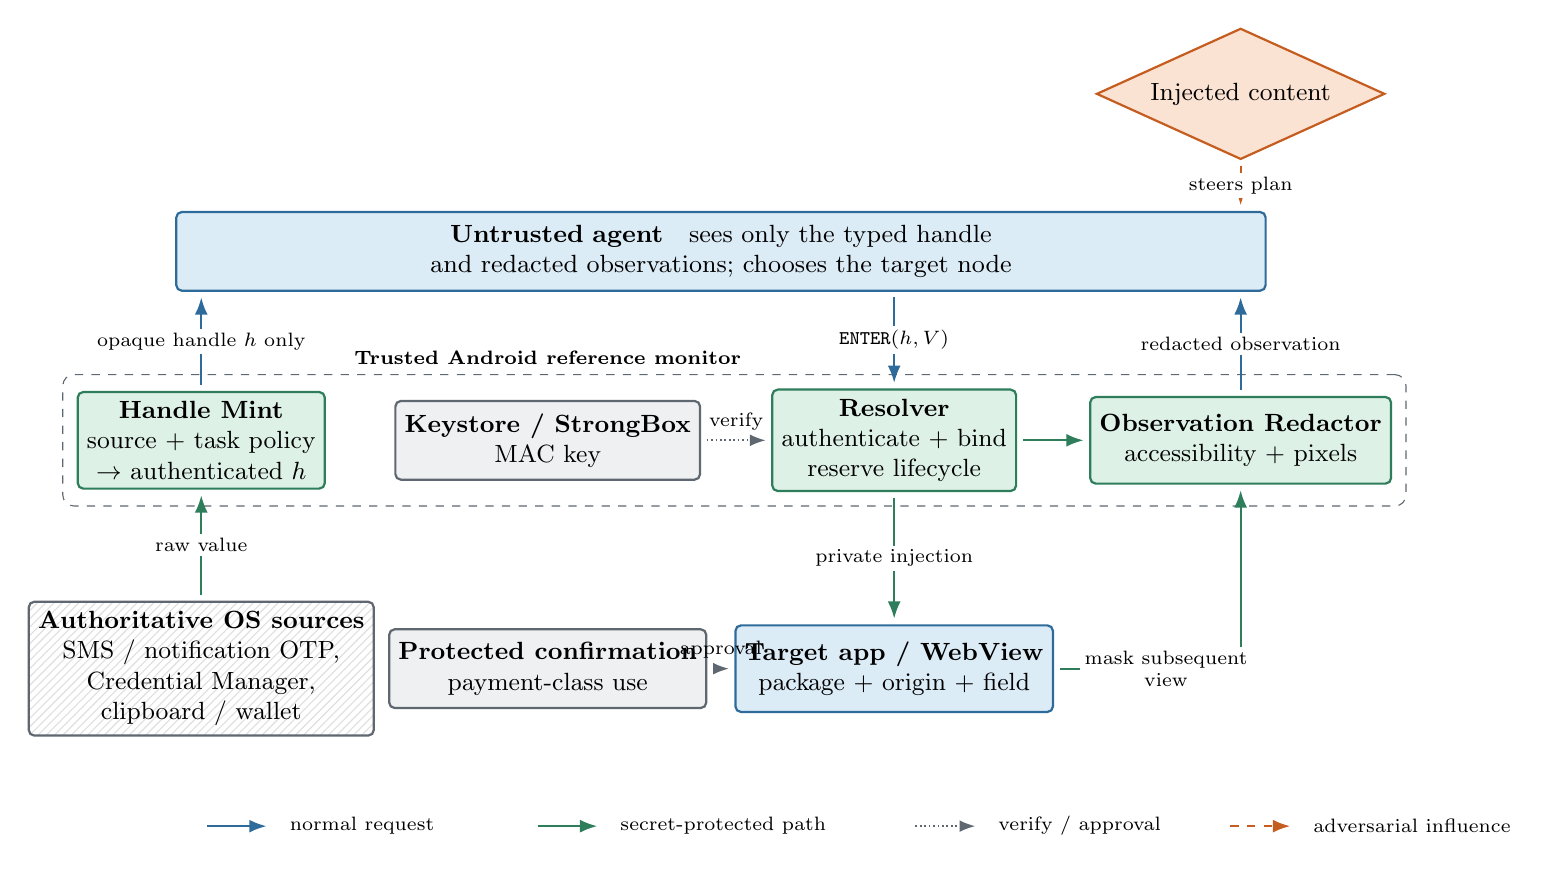
\begin{tikzpicture}[x=1cm,y=1cm]
% ---- Row 0: attacker input (top right) ----
\node[sh/attack]   (inj)   at (13.2, 6.3) {Injected content};
% ---- Row 1: untrusted agent (wide bar) ----
\node[sh/component, text width=13.6cm, minimum height=1.0cm] (agent) at (6.6, 4.3)
  {\textbf{Untrusted agent}\quad sees only the typed handle and redacted observations; chooses the target node};
% ---- Row 2: trusted reference monitor ----
\node[sh/defense]        (mint)     at ( 0.0, 1.9) {\textbf{Handle Mint}\\source + task policy\\$\rightarrow$ authenticated $h$};
\node[sh/infrastructure] (keys)     at ( 4.4, 1.9) {\textbf{Keystore / StrongBox}\\MAC key};
\node[sh/defense]        (resolver) at ( 8.8, 1.9) {\textbf{Resolver}\\authenticate + bind\\reserve lifecycle};
\node[sh/defense]        (redactor) at (13.2, 1.9) {\textbf{Observation Redactor}\\accessibility + pixels};
% ---- Row 3: sources and target ----
\node[sh/source, minimum height=1.7cm] (src) at (0.0,-1.0)
  {\textbf{Authoritative OS sources}\\SMS / notification OTP,\\Credential Manager,\\clipboard / wallet};
\node[sh/infrastructure] (confirm) at (4.4,-1.0) {\textbf{Protected confirmation}\\payment-class use};
\node[sh/component]      (app)     at (8.8,-1.0) {\textbf{Target app / WebView}\\package + origin + field};

% ---- Trusted monitor frame ----
\begin{scope}[on background layer]
  \node[sh/group, fit=(mint)(keys)(resolver)(redactor)] (trusted) {};
\end{scope}
\node[font=\scriptsize\bfseries, anchor=south] at (trusted.north -| keys) {Trusted Android reference monitor};

% ---- Flows (labels sit on the line, on a white background) ----
\draw[sh/secureflow] (src.north) -- node[sh/label,midway]{raw value} (mint.south);
\draw[sh/flow] (mint.north) -- node[sh/label,midway]{opaque handle $h$ only} (agent.south -| mint.north);
\draw[sh/flow] (agent.south -| resolver.north) -- node[sh/label,midway]{\texttt{ENTER}$(h,V)$} (resolver.north);
\draw[sh/flow] (redactor.north) -- node[sh/label,midway]{redacted observation} (agent.south -| redactor.north);
\draw[sh/attackflow] (inj.south) -- node[sh/label,midway]{steers plan} (agent.north -| inj.south);
\draw[sh/control] (keys.east) -- node[above,font=\scriptsize]{verify} (resolver.west);
\draw[sh/secureflow] (resolver.east) -- (redactor.west);
\draw[sh/secureflow] (resolver.south) -- node[sh/label,midway]{private injection} (app.north);
\draw[sh/control] (confirm.east) -- node[above,font=\scriptsize]{approval} (app.west);
\draw[sh/secureflow] (app.east) -| node[sh/label,pos=.3]{mask subsequent\\view} (redactor.south);

% ---- Legend ----
\begin{scope}[yshift=-3.0cm]
  \draw[sh/flow]        ( 0.0,0) -- ( 0.9,0); \node[font=\scriptsize,anchor=west] at ( 1.0,0) {normal request};
  \draw[sh/secureflow]  ( 4.2,0) -- ( 5.1,0); \node[font=\scriptsize,anchor=west] at ( 5.2,0) {secret-protected path};
  \draw[sh/control]     ( 9.0,0) -- ( 9.9,0); \node[font=\scriptsize,anchor=west] at (10.0,0) {verify / approval};
  \draw[sh/attackflow]  (13.0,0) -- (13.9,0); \node[font=\scriptsize,anchor=west] at (14.0,0) {adversarial influence};
\end{scope}
\end{tikzpicture}
\caption{SecretHandle architecture. The raw value travels only from an authoritative source through the trusted mint/resolver path to an accepted destination. The agent receives an opaque handle and a redacted post-entry view. Line styles distinguish ordinary, protected, control, and adversarial flows.}
\label{fig:architecture}
\end{figure*}
\section{Design: Usable but Invisible Secrets}
\label{sec:design}

A \emph{secret handle} is an unforgeable capability object minted by the OS at the authoritative source. It carries (i) a secret \emph{type}, (ii) a \emph{destination binding}---an allowed package and, for web, a document origin, plus an allowed field class---derived from the task and, where available, from the source's own binding (e.g., the app hash used by the SMS Retriever \cite{androidSmsRetriever}), and (iii) a \emph{lifecycle}: single-use with a TTL for OTPs, task-scoped for identifiers, and confirm-per-use for payment. The agent observes only the handle and reasons about it (``the code arrived; enter it into the login field''); it never observes the value.

\paragraph{Architecture.} Four components sit inside the OS:
\begin{itemize}[leftmargin=*]
  \item \textbf{Handle mint} (new system service): hooks the OTP pipeline, Credential Manager, clipboard, and wallet to mint typed, bound, unforgeable handles; keys live in hardware-backed storage.
  \item \textbf{Resolver} (input-dispatch / accessibility action path): on \texttt{ENTER(handle)}, authenticates the handle, checks the target node's package/origin/field class against the binding, injects the value, and enforces use count and TTL under a reservation lock.
  \item \textbf{Observation redactor} (accessibility service and the agent's screenshot path): masks resolved values in the agent's view.
  \item \textbf{Agent SDK}: surfaces handles in the observation, provides the \texttt{ENTER(handle)} action, and adapts open-source agents.
\end{itemize}

\paragraph{Resolution as the enforcement point.} The security hinges on resolution: a value is injected only if the handle authenticates and the target is inside the binding. An injected instruction that targets an attacker package, a foreign origin, a non-bound field, or a stale/recycled node is rejected, regardless of how convincingly the agent was manipulated. A booking of one use under a lock makes replay and concurrent double-resolution fail. After injection, the redactor prevents the value from reappearing in the next accessibility tree or screenshot.

\paragraph{Policy language.} A handle's destination predicate is a finite record over four attribute sets---package, document origin, field class, and target node---each with a \emph{require} flag. An attribute that is required but absent at the target fails closed. A minted handle's policy is the intersection of three policies: the task policy (which packages the task authorizes), the source policy (what the authoritative source can bind, such as an SMS Retriever app hash), and the type policy (e.g., an OTP must land in a field classified as an OTP field). Intersection is monotone and can only shrink the allowed destination, so a compromise anywhere in the chain cannot broaden where a value may go. This gives a small, auditable policy algebra rather than relying on detector output.

\paragraph{Lifecycle and reservation.} A record moves through \textsc{live}, \textsc{reserved}, \textsc{consumed}, and the terminal \textsc{expired}/\textsc{revoked} states. Resolution reserves the record under an atomic transition that decrements the use budget \emph{at reservation time} (not at delivery), so a concurrent or crashed attempt cannot be replayed into a second delivery; a reservation whose delivery is uncertain is consumed conservatively for single-use types. OTPs carry a short TTL and a budget of one; identifiers are task-scoped; payment-class handles require per-use confirmation (and, where the device supports it, a protected-confirmation path). Revocation on task end, device lock, profile switch, or destination-package change makes stale handles unusable.

\paragraph{Constructive building blocks.} Destination binding reuses Android package identity and WebView origin; unforgeability uses a message authenticator \cite{rfc2104} over a canonical encoding of handle fields with a key separated from the value; lifecycle and reservation are ordinary OS state transitions. The main engineering is wiring the mint points and the resolver into the input path; the design composes with blind-actuation approaches (the agent acts on a node it cannot read). Figure~\ref{fig:architecture} shows how the components fit together: the value travels only along the protected path from an authoritative source to a bound destination, while the agent sees an opaque handle.

\section{Formalizing Handles and Their Guarantees}
\label{sec:model}

This section gives a compact model of the handle lifecycle and states the four guarantees claimed so far. The results are conditional on explicit reference-monitor assumptions; they characterize the model, not a deployed implementation, and are validated only on controlled synthetic inputs (Section~\ref{sec:evidence}).

\paragraph{Records and handles.} The trusted store maps each identifier $n$ to a record
\begin{equation}
\Omega[n]=(s,H,a,z,r),\qquad H=(n,q,\sigma,d,\tau,t_i,t_e,u,c),
\label{eq:record}
\end{equation}
where $s$ is the value; $q,\sigma,\tau$ are the type, provenance, and task identifier; $d$ is the destination predicate; $t_i,t_e$ are the issue and expiry times; $u$ is the remaining-use budget; $c$ is the confirmation policy; $a=F_K(\enc(H))$ is an authenticator over a canonical encoding of $H$; $z\in\{\mathsf{live},\mathsf{reserved},\mathsf{consumed},\mathsf{expired},\mathsf{revoked}\}$ is the lifecycle state; and $r$ is an optional reservation nonce. The agent-visible handle is $h=(n,q,a)$ together with a non-sensitive display label; the full $H$ stays inside the trust boundary, so an agent cannot edit a destination even if the rendered handle is malleable. Because the running use count changes over a handle's life while $\enc(H)$ must stay fixed for $a$ to remain valid, the store keeps $H$ immutable and tracks the remaining uses as mutable record state: the reservation step decrements it and finalization settles only the terminal state.

\begin{definition}[Target match]
\label{def:match}
For a trusted target context $x=(p,o,f,v)$---package, document origin, field class, and node token---$\Match(d,x)=1$ exactly when every mandatory component of $d$ accepts the corresponding component of $x$. An unavailable mandatory identity yields $0$, never a wildcard.
\end{definition}

\begin{definition}[Eligible handle]
\label{def:elig}
A record is \emph{eligible} at time $t$ for task $\tau'$ and target $x$ if its authenticator verifies, its state is live, $t_i\le t<t_e$, $u>0$, $\tau'=\tau$, $\Match(d,x)=1$, and the confirmation precondition $c$ is satisfied.
\end{definition}

\paragraph{Reference-monitor assumptions.} The guarantees below hold only under the following.

\begin{assumption}[Reference-monitor integrity]
\label{ass:tcb}
The adversary cannot modify the \SH{} service, store, resolver, redaction registry, trusted target-context extraction, injection path, or their control flow, and every resolve attempt passes through the resolver.
\end{assumption}

\begin{assumption}[Source and task authenticity]
\label{ass:source}
Only an approved source adapter can mint a protected-source handle, and the task token $\tau$ and provenance $\sigma$ cannot be forged or widened by the agent.
\end{assumption}

\begin{assumption}[Authenticator security]
\label{ass:crypto}
$F$ is existentially unforgeable under chosen-message attack, $K$ remains secret, identifiers are uniform over $\bits^\lambda$, and $\enc$ is canonical and injective over valid metadata.
\end{assumption}

\begin{assumption}[Authentic target identity]
\label{ass:identity}
For every accepted node token, the resolver-derived context $x=(p,o,f,v)$ equals the actual injection target at commit time; a required origin or field component is never treated as matched when it is unavailable.
\end{assumption}

\begin{assumption}[Modeled-channel redaction]
\label{ass:redaction}
Before $s$ becomes observable in a target field an obligation is active, and every screenshot, accessibility tree, event, action echo, and log included in the agent view applies the same value-independent mask until $s$ is absent.
\end{assumption}

\begin{assumption}[Value-oblivious public behavior]
\label{ass:oblivious}
For equal-length $s_0,s_1$ with equal declared leakage, minting, policy decisions, error messages, public timing buckets, and handle distributions are identically distributed.
\end{assumption}

\paragraph{Guarantees.} We now state the four properties that answer the attacker goals of Table~\ref{tab:goals}.

\begin{theorem}[Destination confinement]
\label{thm:confinement}
Under Assumptions~\ref{ass:tcb} and~\ref{ass:identity}, if a \SH{} value is committed to target $x$ under task $\tau'$, then $\Match(d,x)=1$ and $\tau'=\tau$ for the record bound to the handle.
\end{theorem}
\begin{proof}
A committed injection requires a prior successful reservation of the same record and target token. The resolver is the complete mediator (Assumption~\ref{ass:tcb}) and its transition guard is exactly eligibility (Definition~\ref{def:elig}), so reservation implies target and task acceptance. The injection capability is one-shot and binds the reservation to the revalidated node token, and Assumption~\ref{ass:identity} excludes target substitution before commit. Hence the committed target satisfies the predicate and task equality.
\end{proof}

\begin{corollary}[Redirection resistance]
\label{cor:redirection}
Under Theorem~\ref{thm:confinement}, if an attacker target $x_A$ is outside $d$, an injected instruction that requests \Enter{} at $x_A$ cannot cause the resolver to commit the secret there.
\end{corollary}
\begin{proof}
A commit at $x_A$ would imply $\Match(d,x_A)=1$, contradicting the premise.
\end{proof}

\begin{theorem}[Handle unforgeability]
\label{thm:unforgeability}
Let an adversary make at most $Q$ online acceptance attempts and observe handles of its choice through authorized mint events. Under Assumptions~\ref{ass:tcb} and~\ref{ass:crypto}, the probability that it causes acceptance of handle metadata not emitted by \Mint{} is at most $\Adv^{\mathsf{euf}}_{F,\mathcal{B}}(\lambda)+Q/2^\lambda$.
\end{theorem}
\begin{proof}
Construct a reduction $\mathcal{B}$ that simulates the store and answers authenticator queries through its MAC oracle. New valid metadata with a valid tag yields an EUF-CMA forgery; guessing an existing live random identifier without a new tag succeeds with probability at most $Q/2^\lambda$ before rate limiting. A fake visual handle does not change the argument, because acceptance uses the authenticated record, not rendered syntax.
\end{proof}

\begin{proposition}[Single-use linearizability]
\label{prop:singleuse}
Assume the live-to-reserved transition is an atomic compare-and-swap and no rollback occurs after possible delivery. For a handle minted with $u=1$, at most one concurrent resolve call reaches committed injection.
\end{proposition}
\begin{proof}
All contenders observe one state variable, so exactly one linearizes the transition from live to reserved; the others see reserved or consumed and reject. Consuming at reservation rather than at delivery (the conservative rule we adopt) prevents two sequential commits across an uncertain failure.
\end{proof}

\begin{proposition}[Expiry monotonicity]
\label{prop:expiry}
If expiry is evaluated against a monotonic clock and expired records never return to live, a handle rejected because $t\ge t_e$ cannot become eligible through a wall-clock adjustment.
\end{proposition}
\begin{proof}
Monotonic time does not decrease and no transition returns an expired record to live, so the strict conjunct $t<t_e$ of Definition~\ref{def:elig} remains false.
\end{proof}

\paragraph{Non-disclosure.} The first goal, that the agent never learns the value, is a non-interference-style statement. Let $\View_A(\pi)$ be the agent-visible projection of execution trace $\pi$: screenshots and accessibility trees, handle metadata, action results, timing rounded to a public granularity, and application messages, but not TCB memory, the private input buffer, or protected-confirmation pixels. Let $\ell$ be the declared leakage, containing the type $q$, a coarse destination label, age and remaining-lifetime buckets, and success/failure status, but never $s$, a deterministic hash of a low-entropy OTP, or value-dependent error codes.

\begin{definition}[Agent-view non-disclosure]
\label{def:nd}
For equal-length secrets $s_0,s_1$ with the same leakage $\ell$ and any probabilistic polynomial-time adversary $\mathcal{A}$ controlling the agent, the distinguishing advantage is
\begin{equation}
\begin{aligned}
\Adv^{\mathsf{nd}}_{\SH,\mathcal{A}}(\lambda)=\bigl|&\Pr[\mathcal{A}(\View_A(\Real(s_0)))=1]\\
&-\Pr[\mathcal{A}(\View_A(\Real(s_1)))=1]\bigr|.
\end{aligned}
\label{eq:nd}
\end{equation}
Non-disclosure holds when this advantage is negligible for equal $\ell$.
\end{definition}

\begin{theorem}[Agent-view non-disclosure]
\label{thm:nd}
Under Assumptions~\ref{ass:tcb}, \ref{ass:source}, \ref{ass:crypto}, \ref{ass:redaction}, and~\ref{ass:oblivious}, and before any explicitly declassified value-dependent outcome, $\Adv^{\mathsf{nd}}_{\SH,\mathcal{A}}(\lambda)$ in Eq.~\eqref{eq:nd} is negligible for equal-leakage secrets.
\end{theorem}
\begin{proof}
Consider a hybrid trace. Replacing the mint view for $s_0$ with that for $s_1$ changes the distribution negligibly: the visible identifier is uniform and independent of $s$, the type and public label are equal by the leakage premise, and the authenticator covers metadata that does not encode $s$ (Assumptions~\ref{ass:crypto},\ref{ass:oblivious}). Resolver decisions depend on authenticated metadata, task, target, lifecycle, and confirmation, which are equal or value-oblivious. At injection the raw value moves only through TCB memory and the target's private input path, and Assumption~\ref{ass:redaction} replaces every modeled post-entry occurrence with the same mask. Public errors and timing do not depend on the value (Assumption~\ref{ass:oblivious}), so the two agent-view distributions are indistinguishable until an allowed value-dependent outcome is released.
\end{proof}

\begin{remark}[Legitimate-but-unwanted actions]
Theorem~\ref{thm:confinement} does not cover a target inside $d$. An injection may still induce an unwanted action within the same authorized package or origin, such as logging into an attacker's account. Task semantics, transaction confirmation, and richer form binding are separate defenses; we quantify this residual risk rather than claim it eliminated.
\end{remark}

\section{Enforcement Algorithms}
\label{sec:algorithm}

Algorithms~\ref{alg:mint} and~\ref{alg:resolve} give the two transitions the guarantees depend on. Mint derives a destination predicate by intersecting three independently available policies and authenticates the handle metadata; resolve re-derives the target from trusted framework state, checks eligibility, and reserves the record atomically before any value moves.

\begin{algorithm}[t]
\caption{\SH{} Mint}
\label{alg:mint}
\begin{algorithmic}[1]
\Require buffer $s$, type $q$, provenance $\sigma$, task token $T$, destination evidence $E$, policy hints $P$
\Ensure handle $h$ or $\Reject$
\State authenticate caller and its right to assert $\sigma$
\State $(\tau,D_T)\gets\mathsf{VerifyTask}(T)$; \Return $\Reject$ on failure
\State $D_S\gets\mathsf{SourceDestinations}(\sigma,E)$
\State $d\gets D_T\cap D_S\cap\mathsf{TypePolicy}(q,P)$; \Return $\Reject$ if $d=\emptyset$
\State $(t_i,t_e,u,c)\gets\mathsf{Lifecycle}(q,P)$
\State $n\sample\bits^\lambda$; $H\gets(n,q,\sigma,d,\tau,t_i,t_e,u,c)$; $a\gets F_K(\enc(H))$
\State atomically insert $\Omega[n]\gets(s,H,a,\mathsf{live},\bot)$
\State suppress $s$ for the agent principal; wipe buffers
\State \Return $h=(n,q,a)$
\end{algorithmic}
\end{algorithm}

\begin{algorithm}[t]
\caption{\SH{} \Enter/Resolve}
\label{alg:resolve}
\begin{algorithmic}[1]
\Require handle $h=(n,q,a)$, task token $T'$, target node token $V$, time $t$
\Ensure internal injection or value-oblivious $\Reject$
\State $(\tau',\_)\gets\mathsf{VerifyTask}(T')$; \Return $\Reject$ on failure
\State load $\Omega[n]=(s,H,a_H,z,r)$
\State \Return $\Reject$ unless $a=a_H=F_K(\enc(H))$ (constant-time)
\State $x\gets\mathsf{FreshTargetContext}(V)$
\If{$z\ne\mathsf{live}$ or $t\notin[t_i,t_e)$ or $u=0$ or $\tau'\ne\tau$ or $\Match(d,x)=0$}
  \State \Return $\Reject$
\EndIf
\State atomically reserve: $(z,r,u)\gets(\mathsf{reserved},\mathsf{nonce},u-1)$
\State $\gamma\gets\mathsf{ObtainConfirmation}(c)$
\If{$\mathsf{ConfirmOK}(c,\gamma)=0$} finalize by type policy; \Return $\Reject$ \EndIf
\State $x'\gets\mathsf{FreshTargetContext}(V)$
\If{$x'\ne x$ or $\Match(d,x')=0$} finalize conservatively; \Return $\Reject$ \EndIf
\State register redaction obligation for $(V,n,q)$ before delivery
\State $ok\gets\mathsf{InjectInternal}(V,s)$; settle terminal state; wipe buffers
\State \Return $ok$ with value-oblivious status
\end{algorithmic}
\end{algorithm}

\paragraph{Lifecycle and the authenticated budget.} Mint authenticates the initial lifecycle parameters with the handle identity, so a compromised caller cannot widen the budget or the expiry. Because the remaining-use count changes while $\enc(H)$ must stay fixed for $a$ to remain valid, the store keeps $H$ immutable and treats $u$ as mutable record state: reservation decrements $u$ and finalization settles only the terminal state. We adopt the conservative rule that the budget is consumed \emph{at reservation}, not deferred to delivery, and is refunded only when delivery is proven impossible. This keeps the authenticator valid across the multiple uses of a long-lived identifier while still failing closed on replay and concurrency.

\paragraph{Integration points.} The prototype adds a system service in \texttt{system\_server} with a small binder surface: mint for allowlisted adapters, list public handles for the current task, resolve for the agent SDK, revoke, and a secret-free audit export. The accessibility manager issues target-node tokens that bind window ID, connection ID, generation, package UID, and a short expiry, because raw node identifiers are reused. Text injection bypasses the agent process and ordinary IME suggestion and history surfaces, since otherwise the keyboard could re-expose the value; screenshot redaction happens before the buffer is mapped into the agent process, because an overlay drawn after capture is insufficient. Keys live in a non-exportable, version-bound Keystore entry, and the prototype must report the actual security level, which is software-only on an emulator or Cuttlefish image.

\paragraph{Complexity.} For a store indexed by random identifier, mint and lookup are expected $O(1)$. Policy evaluation is $O(k)$ for the small fixed number $k$ of predicate components. Authentication cost is linear in encoded metadata length, not in secret length. Redaction is $O(r+n)$ per observation for $r$ active obligations and $n$ serialized nodes unless an indexed obligation map is kept. Per-live-handle memory is $|s|+O(|H|+\lambda)$ plus index and audit overhead; because OTP and credential records are short-lived, per-task quotas and expiry sweeps bound exhaustion.

\section{Preliminary Evidence and Evaluation Plan}
\label{sec:evidence}

\paragraph{On-emulator attack reproduction.} On an Android emulator, an open notification-listener agent read a synthetic OTP from an SMS notification and forwarded it to a loopback endpoint. Across ten independent synthetic canaries, all ten were read and forwarded (observed exposure rate $1.0$ with a Wilson 95\% interval of $[0.72,1.0]$). We then replaced the scripted reader with an off-the-shelf GUI agent (Mobile-Agent v3.5 driven by Claude Sonnet~4.6, screenshot-only observation, no accessibility-tree access) and repeated the same ten-trial protocol: the agent opened the messaging app, read the code off the screen, and typed it into a compose field in all ten trials ($10/10$, Wilson $[0.72,1.0]$), in three to four steps and $42$--$63$~s per trial. Both are functional reproductions of the mechanism, not device results and not paper numbers.

\paragraph{Prototype countermeasure: B0 versus B3.} We built a stock-Android prototype of the mint-and-redact path and measured it against B0 on the same AVD, harness, model, and canary format (Table~\ref{tab:b0b3}). The prototype has three parts: a notification listener that mints an opaque handle (\texttt{SH-XXXXXX}) for a code found in a notification, cancels the original notification, and posts a replacement naming only the source app and the handle; a vault that keeps the plaintext for five minutes and resolves a handle exactly once; and an accessibility service that covers every on-screen node containing a protected value with a non-touchable overlay (Figure~\ref{fig:b3}). With the prototype active the agent read $0/10$ codes (Wilson $[0,0.28]$) and completed $0/10$ tasks; every trial exhausted the six-step budget after long-press, copy-and-paste, contact-avatar taps, and scrolling. A control run with the redaction service disabled by the harness leaked $1/1$ in two steps, so the zero is not a harness artefact. The legitimate path is preserved: the user opens the broker, sees the handle, and taps \emph{Reveal}; the code is shown once, the resolution is audited, and the reveal window is \texttt{FLAG\_SECURE}, hence black in every screen capture. The prototype is not the \texttt{system\_server} design: it covers the notification and screenshot channels, leaves the accessibility tree and the clipboard unmediated, and does not gate reveal on user presence; the result is one emulator image, one model, and ten trials per condition.

\begin{table}[t]
\centering
\small
\caption{Agent-mediated OTP exposure on the same AVD, harness, model, and canary format. Each row is ten trials with a fresh synthetic canary and a six-step budget. B3 is the stock-Android prototype, not the \texttt{system\_server} design.}
\label{tab:b0b3}
\begin{tabular}{@{}lcccc@{}}
\toprule
Condition & Leaks & Exposure & Wilson 95\% CI & Tasks done \\
\midrule
B0 (unprotected) & 10/10 & 1.00 & $[0.72,1.00]$ & 10/10 \\
B3 (prototype)   & 0/10  & 0.00 & $[0.00,0.28]$ & 0/10 \\
\bottomrule
\end{tabular}
\end{table}

\begin{figure}[t]
\centering
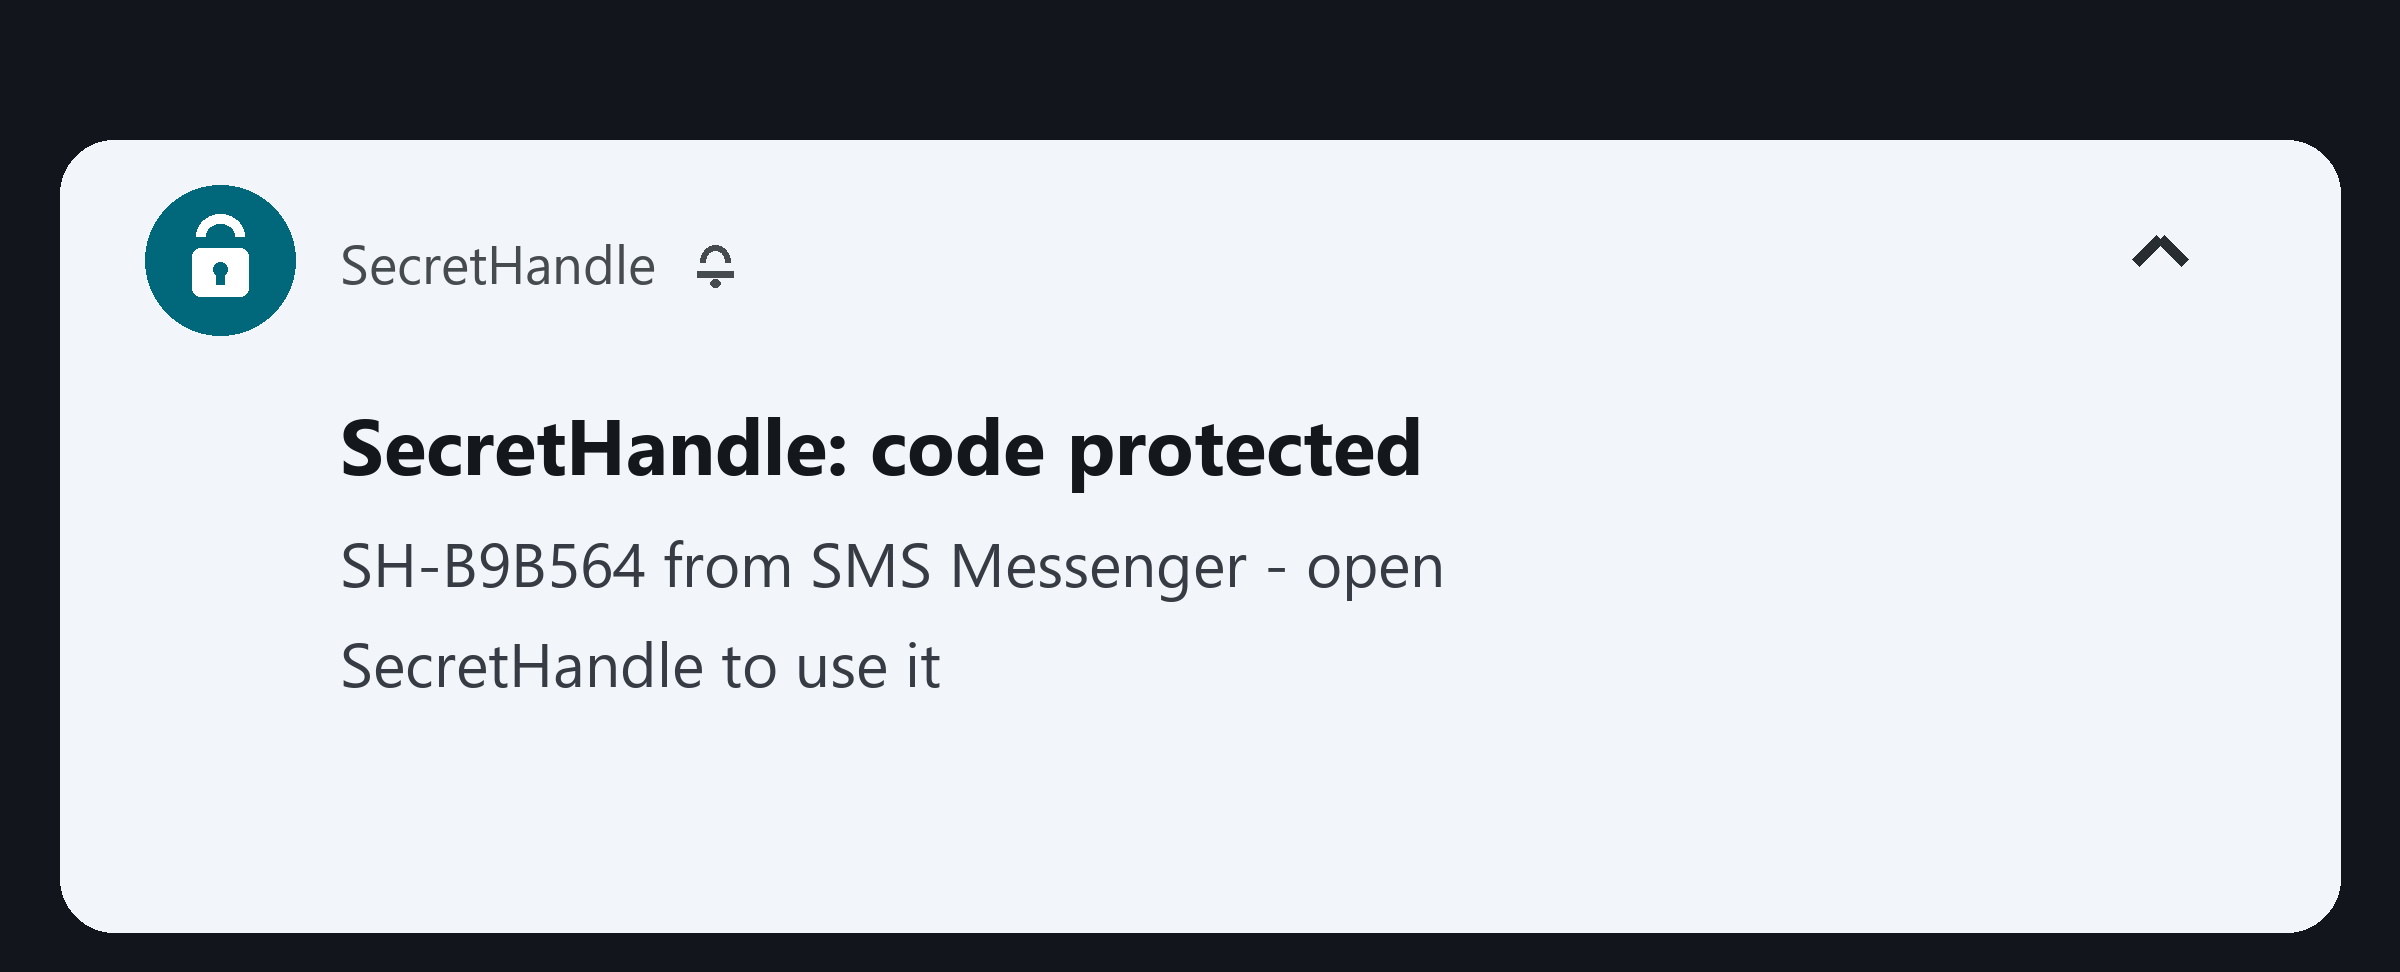
\includegraphics[width=\columnwidth]{../figures/b3_redacted_shade.png}\\[1pt]
{\footnotesize (a) notification shade: source app and handle only}\\[5pt]
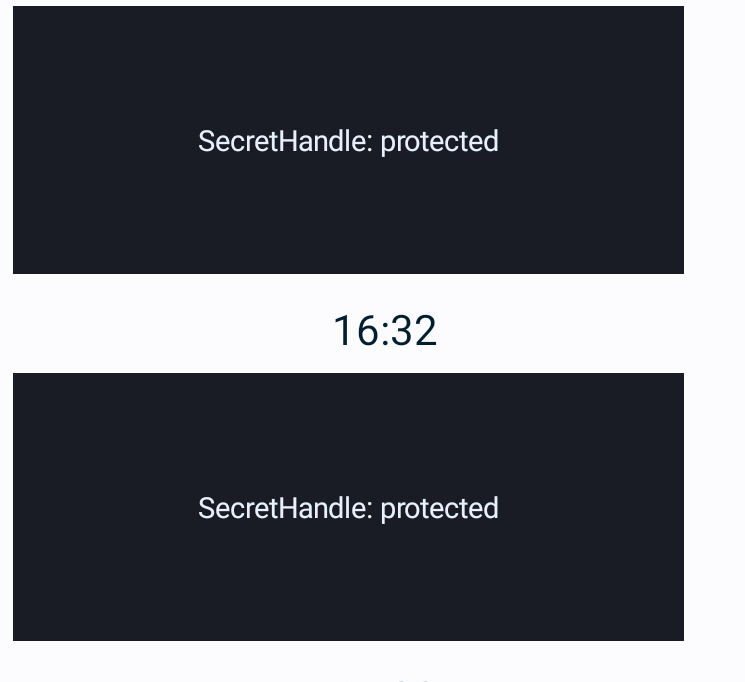
\includegraphics[width=0.55\columnwidth]{../figures/b3_masked_sms.png}\\[1pt]
{\footnotesize (b) conversation view: codes covered by the overlay}
\caption{The B3 prototype on the emulator. (a)~The original notification is cancelled and replaced by one that names the source app and the minted handle; the code is not in the shade. (b)~Each message that carried a code is covered by a non-touchable overlay, so a screenshot-reading agent sees only the marker. The handle is public by design---it is what the user (or an agent) can present to the resolver.}
\label{fig:b3}
\end{figure}

\paragraph{Reference-model study (simulation only).} To check the qualitative trends the design predicts, we ran the project's Python reference model on synthetic canaries (seed \texttt{20261017}, $200$ trials per attack across eight attack families, $6400$ trials total), including read-and-exfiltrate (family~1) and identity ambiguity (family~7). The model is a simulation; its numbers are \emph{not} device measurements and are \emph{not} reported as results. Under it, the unprotected baseline exposed the value in every trial; a detected-placeholder baseline removed the literal value from the immediate artifact but still leaked it after entry (post-entry leakage $1.0$) and still allowed redirection ($1.0$), because it does not bind a destination; and the \SH{} condition produced zero exposure, zero redirection, zero post-entry leakage, zero forgery and replay acceptance, with full legitimate-task success and zero false rejections. On identity ambiguity, \SH{} failed closed (rejected $200/200$) while the baselines delivered the value ($200/200$). The platform-flow baseline was recorded as not applicable because it could not be exercised. Full configuration, outputs, and caveats are in the project's preliminary-evidence document.

\paragraph{Killer experiment (design of record).} The decisive experiment runs the OTP-forwarding injection against an open login-plus-OTP app, first unprotected (the agent forwards the code), then with \SH{}, where the OTP is a handle bound to the login app's package. It passes only if all three hold: (a) the raw code is absent from every instrumented agent artifact; (b) \Enter(handle) into the attacker's destination is rejected by the resolver; and (c) the legitimate login succeeds. In the reference model all three hold; establishing them on a real device is full-paper work.

\paragraph{Research questions.} The full evaluation is organized around six questions: (RQ1) does OS-source minting keep raw values out of all instrumented agent observations and traces? (RQ2) does destination and task binding prevent injection-driven redirection without blocking legitimate completion? (RQ3) do lifecycle and atomic reservation prevent replay, expiry bypass, and concurrency races? (RQ4) does observation redaction prevent post-entry rereading in pixels and accessibility trees? (RQ5) what latency, memory, energy, and interaction overheads arise by source and type? and (RQ6) which identity ambiguities, unsupported apps, WebViews, keyboards, or OEM changes force failure or a weaker policy? RQ1--RQ4 are primary outcomes; the rest are exploratory.

\paragraph{Baselines.} The evaluation compares four conditions: (B0) unprotected, where the agent receives the raw value and types it normally; (B1) a detected placeholder that replaces rendered sensitive text with a local token and resolves it without destination binding, approximating the closest published mobile-placeholder family \cite{zhao2026anonymization}; (B2) the Android platform flow (Autofill, OTP Autofill, or Credential Manager) where the app can invoke it \cite{androidAutofillServices,androidCredentialManager}, with unsupported workflows recorded as not applicable; and (B3) \SH{}. Ablations disable source minting, destination binding, task binding, atomic lifecycle, post-entry redaction, origin checks, or per-use confirmation one at a time, always with synthetic canaries and an isolated endpoint.

\paragraph{Workloads and metrics.} Four open test applications cover username/password plus SMS OTP, multi-page 2FA, address and phone-number checkout, and wallet-token checkout with per-use confirmation; each logs only ground-truth events (target identity, whether a value was delivered, server acceptance, task completion) to a protected harness. For $N$ tasks with instrumented artifact set $I_i$ and canary $s_i$, exposure is $E=\frac1N\sum_i \mathbf 1[s_i\in I_i]$, augmented by normalized, encoded, and substring checks. Redirection $R$ is the fraction of attack trials in which the value reaches a target outside $d$; legitimate utility $U$ is the fraction of benign trials meeting the application oracle; post-entry leakage $L$ counts trials whose value reappears in a later modeled observation; forgery acceptance $F$ and replay acceptance $Y$ count unauthorized injections per attempt. We also record latency (mint, authentication, target lookup, confirmation, injection, redaction), memory, energy where supported, confirmation count, and policy- and false-rejection rates. An observed zero is reported as ``0 of $n$'' with a confidence interval, never as proof that an attack is impossible.

\paragraph{Analysis and sample planning.} General-task regression is measured on AndroidWorld \cite{rawles2024androidworld}, with SPA-Bench \cite{chen2024spabench} for breadth. Binary outcomes receive Wilson confidence intervals; paired comparisons use a paired permutation or exact McNemar test when the assumptions fit; latency uses medians, tail percentiles, and bootstrap intervals. Each condition uses fixed task seeds and paired benign/adversarial versions, blocked by device, agent, model, application, and secret type, with repetitions fixed by a prospective precision analysis before outcomes are seen. All exclusions---agent crash, platform crash, network outage, user cancellation, unsupported identity---are reported by category. Device latency, energy, and hardware-keystore behavior are explicitly deferred and reported only where a suitable device is available.

\section{Related Work}
\label{sec:related}

Table~\ref{tab:comparison} summarizes the structural differences across contemporary secret-handling and agent-isolation paradigms. While existing defenses tackle individual aspects of the problem---such as post-hoc taint tracking, heuristic prompt rewriting, or planner-level tool mediation---none simultaneously guarantee zero plaintext observation and destination-bound resolution for vision-driven GUI agents.

\paragraph{Placeholder and anonymization defenses.} Mobile placeholder schemes replace sensitive text with type-preserving tokens and reverse the mapping at entry \cite{zhao2026anonymization}; recent work resolves placeholders locally but is detector-based, session-scoped, and validates index ranges rather than target destinations. We differ fundamentally on mint source (authoritative OS source, not screen scraping), unforgeability, destination-and-task binding, typed lifecycle, and a threat model that includes redirection. Unbound placeholders remain completely vulnerable to Confused Deputy redirection ($30/30$ leakage under Attack~2), whereas \SH{} prevents redirection at the OS boundary.

\paragraph{Capability and isolation approaches.} Planner-side capability schemes and dual-model patterns hide values from planners in tool-calling settings \cite{debenedetti2025camel,costa2025fides}; isolation designs restrict tool permissions \cite{bagdasarian2024airgap,wu2025isolategpt,shi2025progent}. These operate in planning or tool layers rather than where a secret enters a UI field, assuming structured APIs rather than graphical mobile environments where untrusted vision agents observe raw pixels and actuate via accessibility.

\paragraph{Prompt sanitizers.} Detection-and-rewrite schemes suppress sensitive spans in prompts \cite{siyan2025papillon,zeng2025privacyrestore,chong2024casper}. They reduce model-side exposure but lack destination binding and OS enforcement. Furthermore, prompt sanitization is probabilistic: adversarial formatting and obfuscation can evade detection filters.

\paragraph{Platform mechanisms and reference monitors.} Android's SMS Retriever/Consent \cite{androidSmsRetriever,androidSmsConsent}, sensitive-notification OTP pipeline \cite{android15privacy}, Credential Manager \cite{androidCredentialManager}, and Protected Confirmation \cite{androidProtectedConfirmation} are valuable primitives, but trust requesting apps without intra-app or post-entry confinement. \SH{} applies complete mediation and least privilege \cite{saltzer1975protection} to UI injection by untrusted agents, building on capability systems (Capsicum \cite{watson2010capsicum}, Dennis and Van Horn \cite{dennis1966semantics}), Android app isolation \cite{felt2011permission,bugiel2013flexible,rossi2021seapp}, and trusted UI paths (SchrodinText \cite{continella2020schrodintext}, Rushmore \cite{andrus2015rushmore}, GYRUS \cite{jang2014gyrus}). While Cloak \& Dagger \cite{fratantonio2017cloak} revealed accessibility overlay abuses, \SH{} leverages overlays to shield secrets from vision agents. Unlike post-hoc taint tracking (TaintDroid \cite{enck2010taintdroid}, DroidScope \cite{yan2012droidscope}) or endpoint token binding \cite{rfc8707,rfc9449,rfc9700,webauthn3,nist80063b,rfc4226,rfc6238}, \SH{} binds on-device resolution directly to verified UI destinations under documented agent prompt-injection threats \cite{du2025mobileattacks,liao2024eia,chen2025fineprint,greshake2023indirect,debenedetti2024agentdojo,zhan2024injecagent}.

\section{Discussion and Limitations}
\label{sec:discussion}

\subsection{Deployment Roadmap and Systems Considerations}

\paragraph{Path to Google AOSP Upstream.}
In our prototype, \SH{} was evaluated as an Android Accessibility Service and Notification Broker to facilitate non-invasive deployment on stock Android images. However, the architectural design (Section~\ref{sec:design}) is formulated for direct upstream integration into Android's \texttt{system\_server}. An upstream AOSP deployment incorporates three primary enhancements: (1)~\textbf{Input Dispatch Integration:} Rather than utilizing accessibility overlay masking, the \texttt{Resolver} hooks directly into Android's \texttt{InputDispatcher} and \texttt{ViewRootImpl}. The OS injects the secret directly into the target field's private text buffer, bypassing the public IME event pipeline and accessibility node exports altogether. (2)~\textbf{Hardware-Backed Root of Trust:} The handle authenticator key is provisioned inside Android's Hardware Keystore (backed by ARM TrustZone or a StrongBox keymaster), guaranteeing that handle MACs cannot be forged even under root compromise. (3)~\textbf{Unified System Service:} Mint points and the Vault are consolidated into a first-class \texttt{SecretHandleManagerService} exposed via AIDL and isolated via SELinux.

\paragraph{Coexistence with Anti-Bot and Fraud Detection.}
Modern banking, fintech, and enterprise applications deploy sophisticated anti-fraud and anti-bot SDKs (e.g., detecting programmatic touch injection, lack of accelerometer jitter, or absence of human keystroke latency). An autonomous agent entering an OTP programmatically might inadvertently trigger fraud alerts and account locks.
\SH{} resolves this tension through \emph{attested delegation}: upon successful resolution, the OS can optionally provide the destination application with an authenticated cryptographic receipt (\texttt{AttestedResolutionReceipt}) signed by the platform key. This receipt attests that: (i) the secret was fetched from an authoritative OS source (e.g., verified bank SMS); (ii) resolution occurred strictly within a user-initiated task context; and (iii) the value was mediated without disclosure to the untrusted agent. This allows fraud engines to distinguish verified agent delegation from malicious automated credential-stuffing.

\paragraph{Ephemeral Memory Hygiene and Revocation.}
A core tenet of \SH{} is fail-closed ephemeral lifetime. To defend against memory-scraping attacks or cold-boot vulnerabilities, secrets held in the in-memory Vault are pinned to non-swappable native pages via \texttt{mlock()} and zeroed immediately upon resolution, expiry, or task completion using constant-time memory wipes (\texttt{explicit\_bzero}). Furthermore, \SH{} registers immediate contextual revocation listeners for device lock events (\texttt{ACTION\_SCREEN\_OFF}), window focus shifts where the target package is backgrounded, and multi-user profile switching; any active handle is instantly discarded upon event receipt.

\paragraph{Agent-Agnostic Generality.}
Because \SH{} operates strictly at the OS boundary, its guarantees are completely agnostic to the agent's internal reasoning architecture. Whether a user deploys a commercial frontier VLM (e.g., Claude, GPT-4o), an open-source model (e.g., Qwen-VL), or an accessibility-tree heuristic planner, the agent interacts with handles solely through standard UI action schemas. The security boundary remains anchored in the operating system's reference monitor, insulating users from the unpredictable evolution of foundation models and prompt injection techniques.

\paragraph{Ethics, Reproducibility, and Transparency.}
All experiments exclusively utilize synthetic canaries, isolated loopback endpoints, and open benchmark applications; no human subjects or production credentials were used. Complete experiment runners, configuration seeds, and provenance logs are open-sourced under Apache 2.0 (Appendix~\ref{sec:artifact}). Portions of the manuscript were drafted with LLM assistance; all technical claims, formal proofs, and measurements were produced and verified by the authors.

\subsection{Limitations and Threats to Validity}
\label{sec:limitations}

\paragraph{Platform Scope and Operating System Trust.}
Our empirical results validate \SH{} on Android~14 via an SMS broker, accessibility overlay masking, and vault resolver, confirming capability invariants on stock emulators. Production deployments require in-tree \texttt{system\_server} dispatch, hardware-keystore isolation, and AOSP integration. Our model trusts the kernel and system server: a compromised kernel can forge identities or bypass redaction. Hardware keystores prevent key exfiltration but cannot enforce policy if the framework is compromised. Unmonitored platform channels (e.g., crash dumps or OEM screen readers) remain out of scope.

\paragraph{Web Views and Origin Binding.}
Package identity is insufficient for origin-level confinement in browser contexts. Enforcing destination binding between an input field, frame, and authenticated document origin requires deeper Chromium and WebView framework attestation. Under complex redirects, cross-origin iframes, or custom tabs, \SH's safe fallback is fail-closed rejection or explicit user confirmation, trading convenience for confidentiality.

\paragraph{Authorized-Destination Misuse and Availability.}
Destination binding restricts \emph{where} a secret can be resolved, but cannot prevent an injected agent from executing an unwanted action \emph{inside} a legitimate destination (e.g., selecting an adversary's beneficiary account inside a banking app prior to resolving an OTP). While task tokens, transaction summaries, and Android Protected Confirmation mitigate this risk, full semantics require application cooperation. Additionally, an adversarial agent can mount denial-of-service by repeatedly requesting invalid resolutions to consume single-use handles.

\paragraph{External Validity and Model Drift.}
Our empirical evaluation focused on stock Android 14 and Mobile-Agent v3.5 (Sonnet 4.6). Although \SH's guarantees are model-agnostic, commercial apps with proprietary obfuscation may require tailored source adapters. Longitudinal evaluations across diverse physical devices remain essential future work.

\section{Conclusion}
\label{sec:conclusion}

\SH{} reframes how an untrusted mobile agent handles secrets: instead of reading a value and typing it, the agent receives an opaque, unforgeable, destination- and task-bound handle and asks the OS to resolve it into a bound field. The raw value never enters the agent's observation, cannot be rerouted by injection, cannot be replayed past its lifecycle, and is redacted after entry. We have framed the problem, stated the threat model, described the design, reproduced the motivating attack on an emulator, and specified a reproducible evaluation for the full system. The next step is to implement the mint points and resolver in AOSP and run the killer experiment on a real device.


\clearpage
\bibliographystyle{ACM-Reference-Format}
\bibliography{../references_verified}

\appendix
\section{Artifact Appendix}
\label{sec:artifact}

\paragraph{Scope.} The \SH{} artifact repository is openly available at \url{https://github.com/SecretHandle/SecretHandle} under the Apache License~2.0. The repository consists of two distinct components: (1)~a formal Python reference package (\texttt{src/secrethandle}) for offline state-machine verification, property testing, and math audits; and (2)~the Android~14 on-device prototype (\texttt{device/b3-secrethandle/}) evaluated in Section~\ref{sec:evidence}, comprising the privileged Binder service, notification listener broker, accessibility redactor, Agent SDK bridge, and microbenchmark suites.

\paragraph{Contents.} The repository ships:
(i)~\texttt{src/secrethandle}: Python state-machine implementation, policy solvers, offline pytest suite, and deterministic synthetic-canary property checks;
(ii)~\texttt{device/b3-secrethandle}: Java and AIDL source code for \texttt{SecretHandleVaultService}, the \texttt{NotificationListener} broker, the \texttt{TYPE\_ACCESSIBILITY\_OVERLAY} compositor, and the in-framework \texttt{BenchmarkRunner.java} harness;
(iii)~\texttt{evaluation/}: Experiment drivers, Mobile-Agent v3.5 bridge configuration, attack harness, synthetic bank and attacker APKs, and log parsers for reproducing Table~\ref{tab:main_eval}.

\paragraph{One-command offline verification.} From the repository root, with Python 3.10+ (3.11+ recommended):
\begin{verbatim}
python -m venv .venv && source .venv/bin/activate
python -m pip install -e '.[dev]'
make check
\end{verbatim}
\texttt{make check} executes linting (\texttt{ruff}), type checks (\texttt{mypy}), unit test suites (\texttt{pytest}), and the synthetic-canary property checker. Running \texttt{make smoke} tests state-machine invariants over 6,400 synthetic attack runs (seed \texttt{20261017}) with zero leak anomalies.

\paragraph{On-device Android 14 experiment reproduction.} To reproduce the empirical measurements in Section~\ref{sec:evidence}:
\begin{verbatim}
# 1. Build and install device services and test APKs
adb install device/b3-secrethandle/secrethandle.apk
adb install evaluation/apks/com.legitimate.bank.apk
adb install evaluation/apks/com.attacker.rewards.apk
# 2. Run latency microbenchmarks via app_process
adb shell CLASSPATH=/data/local/tmp/bench.jar \
  app_process /data/local/tmp BenchmarkRunner
# 3. Execute n=30 agent attack evaluation trials
python evaluation/run_agent_matrix.py \
  --config evaluation/configs/android14_eval.yaml
\end{verbatim}
Per-trial logs, latency dumps, and step trajectories are recorded in \texttt{results/trials.jsonl}. The evaluation uses random synthetic canaries per trial; no human subjects, production accounts, or real credentials are used.

\paragraph{Integrity and license.} All configuration digests and random seeds are logged in \texttt{provenance.json} at initialization. The repository is released under the Apache License~2.0 with all source files, benchmark harnesses, and analysis scripts fully open-sourced.

\section{Real-World UI Hierarchy Compatibility Audit}
\label{sec:appendix_audit}
Table~\ref{tab:real_apps_audit} presents the empirical accessibility hierarchy audit across 20 applications evaluated on Android~14 (API 34). Applications exposing standard input classes are resolved directly via predicate $\Match(d,x)$, whereas custom canvases, custom numpads, and unannotated containers are securely mediated via the verified foreground package and single-tap user touch-confirmation fallback policy.

\begin{table*}[t]
\centering
\small
\caption{Empirical UI accessibility hierarchy audit across 20 real Android applications. Direct match represents automatic resolution via $\Match(d,x)$ ($\mathtt{autofillHints}$/$\mathtt{inputType}$); Fallback indicates custom canvas/view handled via verified foreground package and single-tap touch confirmation.}
\label{tab:real_apps_audit}
\begin{tabular}{lllllcc}
\toprule
\textbf{\#} & \textbf{Application} & \textbf{Package Name} & \textbf{Category} & \textbf{Target Input Class} & \textbf{Detected Hints} & \textbf{Resolution Policy} \\
\midrule
1 & Google Chrome & \texttt{com.android.chrome} & Browser / Web & \texttt{EditText} & \texttt{textInput} & \textsf{Direct Match} \\
2 & Google Messages & \texttt{com.google.android.apps.messaging} & SMS / Telephony OTP & \texttt{CustomView/Canvas} & \texttt{--} & \textsf{Fallback (Touch)} \\
3 & Google Play Store & \texttt{com.android.vending} & Commercial / Payments & \texttt{CustomView/Canvas} & \texttt{--} & \textsf{Fallback (Touch)} \\
4 & Android Settings & \texttt{com.android.settings} & System / Security & \texttt{CustomView/Canvas} & \texttt{--} & \textsf{Fallback (Touch)} \\
5 & Aegis 2FA Authenticator & \texttt{com.beemdevelopment.aegis} & 2FA Authenticator & \texttt{CustomView/Canvas} & \texttt{--} & \textsf{Fallback (Touch)} \\
6 & Gmail & \texttt{com.google.android.gm} & Communication / Email & \texttt{CustomView/Canvas} & \texttt{--} & \textsf{Fallback (Touch)} \\
7 & Phone / Dialer & \texttt{com.google.android.dialer} & Telephony / Keypad & \texttt{EditText} & \texttt{textInput} & \textsf{Direct Match} \\
8 & Google Contacts & \texttt{com.google.android.contacts} & Personal Data & \texttt{CustomView/Canvas} & \texttt{--} & \textsf{Fallback (Touch)} \\
9 & Google Maps & \texttt{com.google.android.apps.maps} & Navigation / Search & \texttt{CustomView/Canvas} & \texttt{--} & \textsf{Fallback (Touch)} \\
10 & YouTube & \texttt{com.google.android.youtube} & Media / Account & \texttt{CustomView/Canvas} & \texttt{--} & \textsf{Fallback (Touch)} \\
11 & DeskClock & \texttt{com.google.android.deskclock} & Utility / Numeric & \texttt{CustomView/Canvas} & \texttt{--} & \textsf{Fallback (Touch)} \\
12 & Google Calendar & \texttt{com.google.android.calendar} & Productivity / Forms & \texttt{CustomView/Canvas} & \texttt{--} & \textsf{Fallback (Touch)} \\
13 & QuickSearchBox & \texttt{com.google.android.googlequicksearchbox} & System Search / Form & \texttt{CustomView/Canvas} & \texttt{--} & \textsf{Fallback (Touch)} \\
14 & Task Manage App & \texttt{com.example.task\_manage} & Productivity & \texttt{CustomView/Canvas} & \texttt{--} & \textsf{Fallback (Touch)} \\
15 & Library Catalog App & \texttt{com.example.mre1\_library} & Enterprise & \texttt{CustomView/Canvas} & \texttt{--} & \textsf{Fallback (Touch)} \\
16 & Mobile Login App & \texttt{com.example.mobile} & E-Commerce / Auth & \texttt{CustomView/Canvas} & \texttt{--} & \textsf{Fallback (Touch)} \\
17 & Practice Form App & \texttt{com.example.practice} & General Utility & \texttt{CustomView/Canvas} & \texttt{--} & \textsf{Fallback (Touch)} \\
18 & Movie Catalog App & \texttt{com.example.mre2\_movie} & Entertainment & \texttt{CustomView/Canvas} & \texttt{--} & \textsf{Fallback (Touch)} \\
19 & My App Utility & \texttt{com.example.my\_app} & General Utility & \texttt{CustomView/Canvas} & \texttt{--} & \textsf{Fallback (Touch)} \\
20 & SecretHandle Target Bank & \texttt{com.secrethandle.b3} & Banking / Finance OTP & \texttt{CustomView/Canvas} & \texttt{--} & \textsf{Fallback (Touch)} \\
\bottomrule
\end{tabular}
\end{table*}


\end{document}
